
\documentclass{standalone}
\usepackage{tikz}


\usetikzlibrary{arrows}
\usetikzlibrary{backgrounds}
\usetikzlibrary{fit}
\usetikzlibrary{positioning}
\usetikzlibrary{patterns}
\usetikzlibrary{shapes}
\usetikzlibrary{shapes.misc}

\tikzset{
  node distance= 0.5cm and 1cm,
  > = stealth,
  data/.style = {rectangle,
                 draw,
                 align = center,
                 text width = 5cm,
                 font = \small,
                 minimum height = 1.5cm,
                 inner sep = 0.05cm},
  function/.style = {rectangle,
                     font = \small\sffamily,
                     minimum width = 1.8cm}
}

\let\code=\texttt

\begin{document}
\centering
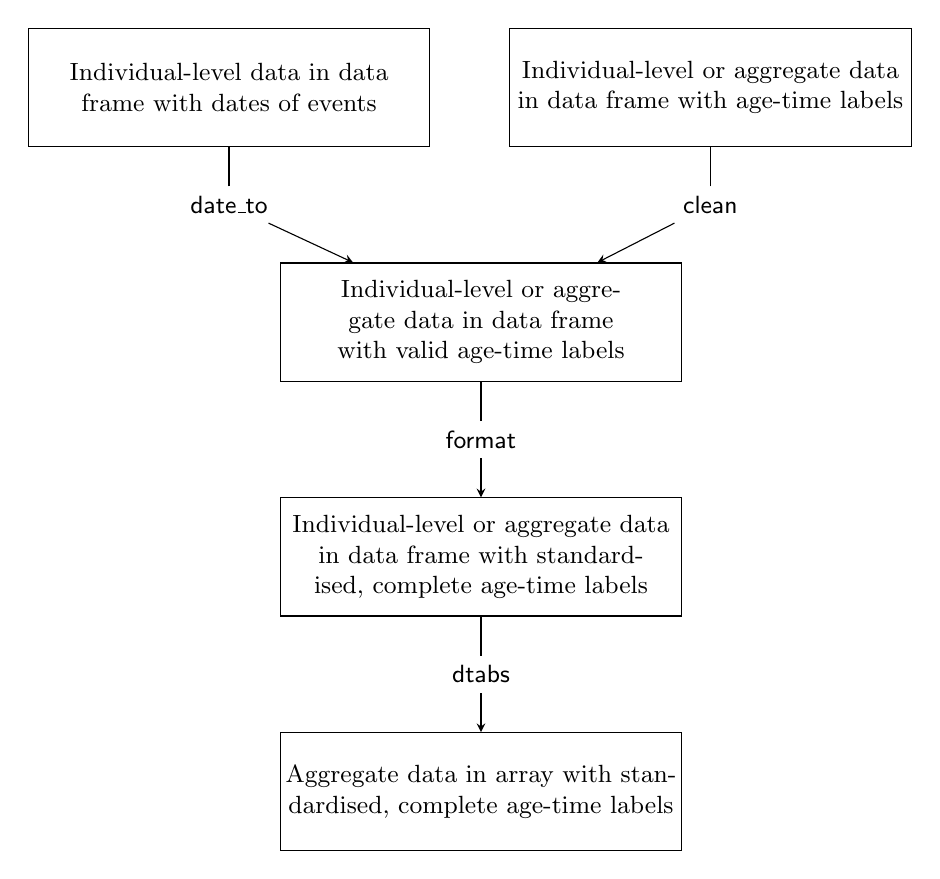
\begin{tikzpicture}

\node[data](data-dates)[]{Individual-level data in data frame with dates of events};

\node[data](data-ag)[right = of data-dates]{Individual-level or aggregate data in data frame with age-time labels};

\node[function](date-to)[below = of data-dates]{date\_to}
  edge[-](data-dates);
  
\node[function](clean)[below = of data-ag]{clean}
  edge[-](data-ag);

\node[data](data-clean)[below = of date-to, xshift = 3.2cm]{Individual-level or aggregate data in data frame with valid age-time labels}
  edge[<-](date-to) edge[<-](clean);

\node[function](format)[below = of data-clean]{format}
  edge[-](data-clean);
  
\node[data](data-format)[below = of format]{Individual-level or aggregate data in data frame with standardised, complete age-time labels}
  edge[<-](format);
  
\node[function](dtabs)[below = of data-format]{dtabs}
  edge[-](data-format);
  
\node[data](data-tab)[below = of dtabs]{Aggregate data in array with standardised, complete age-time labels}
  edge[<-](dtabs);

\end{tikzpicture}

\end{document}
